\newpage
\section{Lecture 3: Likelihood, Loss Functions, and Probabilistic Outputs}

\subsection{Continuation from Shallow to Deep Models}
Recall the shallow mapping
\[
\mathbf{x}\longmapsto y,\qquad y=f(\mathbf{x};\boldsymbol{\phi}).
\]
Deep neural networks are models with more than one hidden layer.

First hidden layer in vector form:
\[
\mathbf{h}^{(1)} = a\!\left(\boldsymbol{\beta}_0+\Omega_0\mathbf{x}\right).
\]
Each hidden unit is a weighted combination of input variables, followed by a
nonlinearity.

\subsection{Dimension Check for Matrix Multiplication}
To ensure multiplication is valid, keep dimensions explicit:
\[
\mathbf{x}\in\mathbb{R}^{d_0},\quad
\Omega_0\in\mathbb{R}^{D_1\times d_0},\quad
\boldsymbol{\beta}_0\in\mathbb{R}^{D_1},\quad
\mathbf{h}^{(1)}\in\mathbb{R}^{D_1}.
\]
Then
\[
\Omega_0\mathbf{x}\in\mathbb{R}^{D_1},
\]
so adding $\boldsymbol{\beta}_0$ is dimensionally correct.

For deeper layers:
\[
\mathbf{h}^{(k)} = a\!\left(\boldsymbol{\beta}_{k-1}+\Omega_{k-1}\mathbf{h}^{(k-1)}\right),
\]
with
\[
\Omega_{k-1}\in\mathbb{R}^{D_k\times D_{k-1}},
\quad
\boldsymbol{\beta}_{k-1}\in\mathbb{R}^{D_k}.
\]

\subsection{Loss Functions and Best Parameters}
Training means finding parameters that best explain data.
Given
\[
\mathcal{D}=\{(\mathbf{x}_i,y_i)\}_{i=1}^{I},
\]
we optimize a loss
\[
L(\mathcal{D},\boldsymbol{\phi})=\sum_{i=1}^{I}\ell\!\left(y_i,f(\mathbf{x}_i;\boldsymbol{\phi})\right).
\]

\subsection{Maximum Likelihood Principle}
In probabilistic modeling, we use conditional probability
\[
p(y_i\mid \mathbf{x}_i,\boldsymbol{\phi}).
\]
Assuming independent observations:
\[
p(y_1,\dots,y_I\mid \mathbf{x}_1,\dots,\mathbf{x}_I,\boldsymbol{\phi})
=
\prod_{i=1}^{I}p(y_i\mid \mathbf{x}_i,\boldsymbol{\phi}).
\]
Maximum likelihood estimator:
\[
\hat{\boldsymbol{\phi}}
=
\arg\max_{\boldsymbol{\phi}}
\prod_{i=1}^{I}p(y_i\mid \mathbf{x}_i,\boldsymbol{\phi}).
\]

Take log (monotonic transform):
\[
\hat{\boldsymbol{\phi}}
=
\arg\max_{\boldsymbol{\phi}}
\sum_{i=1}^{I}\log p(y_i\mid \mathbf{x}_i,\boldsymbol{\phi}).
\]
Equivalent minimization:
\[
\hat{\boldsymbol{\phi}}
=
\arg\min_{\boldsymbol{\phi}}
\left[
-\sum_{i=1}^{I}\log p(y_i\mid \mathbf{x}_i,\boldsymbol{\phi})
\right].
\]

\subsection{From Gaussian Likelihood to Least Squares}
For regression, assume
\[
y_i\mid \mathbf{x}_i,\boldsymbol{\phi}
\sim
\mathcal{N}\!\left(f(\mathbf{x}_i;\boldsymbol{\phi}),\sigma^2\right).
\]
Then
\[
p(y_i\mid \mathbf{x}_i,\boldsymbol{\phi})
=
\frac{1}{\sqrt{2\pi}\sigma}
\exp\!\left(
-\frac{(y_i-f(\mathbf{x}_i;\boldsymbol{\phi}))^2}{2\sigma^2}
\right).
\]
Negative log-likelihood over dataset:
\[
-\sum_{i=1}^{I}\log p(y_i\mid \mathbf{x}_i,\boldsymbol{\phi})
=
\frac{I}{2}\log(2\pi\sigma^2)
+
\frac{1}{2\sigma^2}
\sum_{i=1}^{I}(y_i-f(\mathbf{x}_i;\boldsymbol{\phi}))^2.
\]
Since constants do not depend on $\boldsymbol{\phi}$:
\[
\hat{\boldsymbol{\phi}}
=
\arg\min_{\boldsymbol{\phi}}
\sum_{i=1}^{I}(y_i-f(\mathbf{x}_i;\boldsymbol{\phi}))^2.
\]
So least squares is MLE under Gaussian noise with mean $\mu=f(\mathbf{x};\boldsymbol{\phi})$
and standard deviation $\sigma$.

\subsection{Diagram: Slope-Based Regression (Least Squares)}
\begin{figure}[h!]
\centering
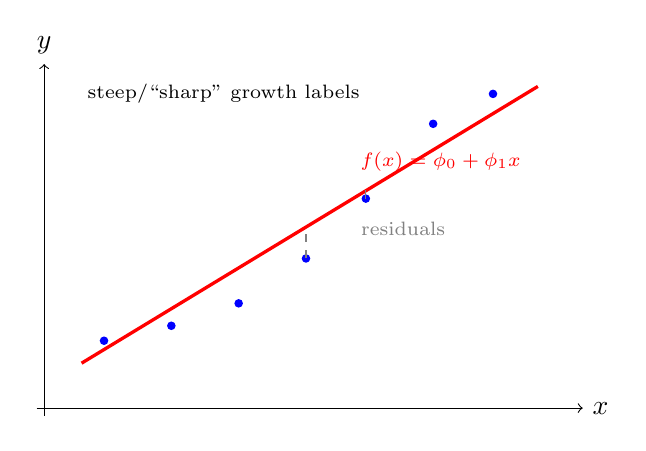
\begin{tikzpicture}[scale=0.95]
    % Axes
    \draw[->] (-0.1,0) -- (7.2,0) node[right] {$x$};
    \draw[->] (0,-0.1) -- (0,4.6) node[above] {$y$};

    % Data points with sharp growth trend
    \filldraw[blue] (0.8,0.9) circle (1.4pt);
    \filldraw[blue] (1.7,1.1) circle (1.4pt);
    \filldraw[blue] (2.6,1.4) circle (1.4pt);
    \filldraw[blue] (3.5,2.0) circle (1.4pt);
    \filldraw[blue] (4.3,2.8) circle (1.4pt);
    \filldraw[blue] (5.2,3.8) circle (1.4pt);
    \filldraw[blue] (6.0,4.2) circle (1.4pt);

    % Linear predictor
    \draw[very thick,red] (0.5,0.6) -- (6.6,4.3);
    \node[red] at (5.3,3.3) {\scriptsize $f(x)=\phi_0+\phi_1x$};

    % Residuals
    \draw[dashed,gray] (4.3,2.8) -- (4.3,3.0);
    \draw[dashed,gray] (3.5,2.0) -- (3.5,2.4);
    \node[gray] at (4.8,2.4) {\scriptsize residuals};
    \node at (2.4,4.2) {\scriptsize steep/``sharp'' growth labels};
\end{tikzpicture}
\caption{Least-squares line fit to data with increasing slope trend.}
\end{figure}

\subsection{Binary Classification and Bernoulli Likelihood}
For binary targets $y\in\{0,1\}$ and Bernoulli parameter $\lambda$:
\[
p(y\mid \lambda)=
\begin{cases}
1-\lambda, & y=0,\\
\lambda, & y=1.
\end{cases}
\]
Equivalent compact form:
\[
p(y\mid\lambda)=(1-\lambda)^{1-y}\lambda^{y},
\qquad
\lambda\in[0,1].
\]

Use a network score $f(\mathbf{x};\boldsymbol{\phi})$ and map it with sigmoid:
\[
\hat{\lambda}=\sigma(f(\mathbf{x};\boldsymbol{\phi})),
\qquad
\sigma(z)=\frac{1}{1+\exp(-z)}.
\]

\subsection{Diagram: Probability Growth with Sigmoid}
\begin{figure}[h!]
\centering
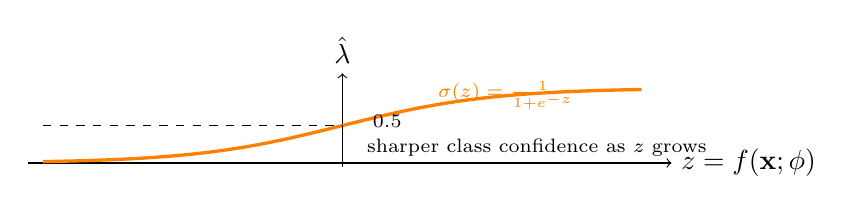
\begin{tikzpicture}[scale=0.95]
    % Axes
    \draw[->] (-4.2,0) -- (4.4,0) node[right] {$z=f(\mathbf{x};\boldsymbol{\phi})$};
    \draw[->] (0,-0.05) -- (0,1.2) node[above] {$\hat{\lambda}$};

    % Sigmoid curve
    \draw[very thick,orange,domain=-4:4,samples=100]
        plot (\x,{1/(1+exp(-\x))});

    % Midpoint marker
    \draw[dashed] (0,0) -- (0,0.5);
    \draw[dashed] (-4,0.5) -- (0,0.5);
    \node at (0.6,0.56) {\scriptsize $0.5$};
    \node[orange] at (2.2,0.9) {\scriptsize $\sigma(z)=\frac{1}{1+e^{-z}}$};
    \node at (2.6,0.2) {\scriptsize sharper class confidence as $z$ grows};
\end{tikzpicture}
\caption{Sigmoid converts score to Bernoulli probability.}
\end{figure}

\subsection{Multiclass Classification and Softmax}
For $K$ classes with logits $f_k(\mathbf{x};\boldsymbol{\phi})$:
\[
p(y=k\mid \mathbf{x},\boldsymbol{\phi})
=
\operatorname{softmax}_k(\mathbf{f}(\mathbf{x};\boldsymbol{\phi}))
=
\frac{\exp(f_k(\mathbf{x};\boldsymbol{\phi}))}
{\sum_{j=1}^{K}\exp(f_j(\mathbf{x};\boldsymbol{\phi}))}.
\]

\subsection{Cross-Entropy as Negative Log-Likelihood}
For one-hot target vector $\mathbf{t}_i$ and predicted class probabilities
$\hat{\mathbf{p}}_i$:
\[
\mathcal{L}_{\mathrm{CE}}
=
-\sum_{i=1}^{I}\sum_{k=1}^{K} t_{ik}\log \hat{p}_{ik}.
\]
This is exactly the negative log-likelihood for categorical outputs.

\subsection{Theoretical vs Empirical Distribution and KL}
Let $p^\star$ be the true (theoretical) data distribution and $\hat{p}_{\text{emp}}$
the empirical distribution from samples.
Cross-entropy decomposition:
\[
H(p^\star,\hat{p}_\phi)
=
H(p^\star)+D_{\mathrm{KL}}(p^\star\parallel \hat{p}_\phi),
\]
where
\[
D_{\mathrm{KL}}(p\parallel q)=\sum_x p(x)\log\frac{p(x)}{q(x)}.
\]
Since $H(p^\star)$ is constant in $\phi$, minimizing cross-entropy minimizes
KL divergence to the target distribution.

\subsection{Dirac Delta View of Empirical Distribution}
For continuous data $\{\mathbf{x}_i\}_{i=1}^{I}$:
\[
\hat{p}_{\text{emp}}(\mathbf{x})
=
\frac{1}{I}\sum_{i=1}^{I}\delta(\mathbf{x}-\mathbf{x}_i),
\]
where $\delta(\cdot)$ is the Dirac delta function.
This formalizes empirical distribution as probability mass concentrated on observed
samples.
